\documentclass[12pt,a4paper]{article}

\usepackage[rmargin=1.2in,lmargin=1.2in,tmargin=.8in,bmargin=.8in]{geometry}
\usepackage{indentfirst}

% fonts
% \usepackage{mathptmx}
\usepackage{fontspec}
\setmainfont{Times New Roman}

% images, table and colors
\usepackage[dvipsnames]{xcolor}
\usepackage{graphicx} 
\graphicspath{ {./figures/} } 
\usepackage{tabularx, makecell}
\usepackage{caption}
\usepackage{subcaption}
\usepackage{enumitem}
\usepackage[normalem]{ulem}

% math support
\usepackage{amsmath}
\usepackage{amssymb,stackengine}

% citations
\usepackage[colorlinks=true,allcolors=blue]{hyperref}
\usepackage[citestyle=authoryear-icomp,bibstyle=authoryear,hyperref=true,
  isbn=false,url=false,eprint=false, giveninits=true, uniquename=init, 
  date=year,maxcitenames=2,uniquelist=minyear,sorting=nyt]{biblatex}
\addbibresource{intern25_ref.bib}
%
%  These Macros are taken from the AAS TeX macro package version 5.2
%  and are compatible with the macros in the A&A document class
%  version 7.0
%  Include this file in your LaTeX source only if you are not using
%  the AAS TeX macro package or the A&A document class and need to
%  resolve the macro definitions in the TeX/BibTeX entries returned by
%  the ADS abstract service.
%
%  If you plan not to use this file to resolve the journal macros
%  rather than the whole AAS TeX macro package, you should save the
%  file as ``aas_macros.sty'' and then include it in your LaTeX paper
%  by using a construct such as:
%	\documentstyle[11pt,aas_macros]{article}
%
%  For more information on the AASTeX and A&A packages, please see:
%       http://journals.aas.org/authors/aastex.html	
%       ftp://ftp.edpsciences.org/pub/aa/readme.html
%  For more information about ADS abstract server, please see:
%       http://adsabs.harvard.edu/ads_abstracts.html
%

% Abbreviations for journals.  The object here is to provide authors
% with convenient shorthands for the most "popular" (often-cited)
% journals; the author can use these markup tags without being concerned
% about the exact form of the journal abbreviation, or its formatting.
% It is up to the keeper of the macros to make sure the macros expand
% to the proper text.  If macro package writers agree to all use the
% same TeX command name, authors only have to remember one thing, and
% the style file will take care of editorial preferences.  This also
% applies when a single journal decides to revamp its abbreviating
% scheme, as happened with the ApJ (Abt 1991).

\makeatletter
\let\jnl@style=\rm
\def\ref@jnl#1{{\jnl@style#1}}

\def\aj{\ref@jnl{AJ}}                   % Astronomical Journal
\def\actaa{\ref@jnl{Acta Astron.}}      % Acta Astronomica
\def\araa{\ref@jnl{ARA\&A}}             % Annual Review of Astron and Astrophys
\def\apj{\ref@jnl{ApJ}}                 % Astrophysical Journal
\def\apjl{\ref@jnl{ApJ}}                % Astrophysical Journal, Letters
\def\apjs{\ref@jnl{ApJS}}               % Astrophysical Journal, Supplement
\def\ao{\ref@jnl{Appl.~Opt.}}           % Applied Optics
\def\apss{\ref@jnl{Ap\&SS}}             % Astrophysics and Space Science
\def\aap{\ref@jnl{A\&A}}                % Astronomy and Astrophysics
\def\aapr{\ref@jnl{A\&A~Rev.}}          % Astronomy and Astrophysics Reviews
\def\aaps{\ref@jnl{A\&AS}}              % Astronomy and Astrophysics, Supplement
\def\azh{\ref@jnl{AZh}}                 % Astronomicheskii Zhurnal
\def\baas{\ref@jnl{BAAS}}               % Bulletin of the AAS
\def\bac{\ref@jnl{Bull. astr. Inst. Czechosl.}}
                % Bulletin of the Astronomical Institutes of Czechoslovakia 
\def\caa{\ref@jnl{Chinese Astron. Astrophys.}}
                % Chinese Astronomy and Astrophysics
\def\cjaa{\ref@jnl{Chinese J. Astron. Astrophys.}}
                % Chinese Journal of Astronomy and Astrophysics
\def\icarus{\ref@jnl{Icarus}}           % Icarus
\def\jcap{\ref@jnl{J. Cosmology Astropart. Phys.}}
                % Journal of Cosmology and Astroparticle Physics
\def\jrasc{\ref@jnl{JRASC}}             % Journal of the RAS of Canada
\def\memras{\ref@jnl{MmRAS}}            % Memoirs of the RAS
\def\mnras{\ref@jnl{MNRAS}}             % Monthly Notices of the RAS
\def\na{\ref@jnl{New A}}                % New Astronomy
\def\nar{\ref@jnl{New A Rev.}}          % New Astronomy Review
\def\pra{\ref@jnl{Phys.~Rev.~A}}        % Physical Review A: General Physics
\def\prb{\ref@jnl{Phys.~Rev.~B}}        % Physical Review B: Solid State
\def\prc{\ref@jnl{Phys.~Rev.~C}}        % Physical Review C
\def\prd{\ref@jnl{Phys.~Rev.~D}}        % Physical Review D
\def\pre{\ref@jnl{Phys.~Rev.~E}}        % Physical Review E
\def\prl{\ref@jnl{Phys.~Rev.~Lett.}}    % Physical Review Letters
\def\pasa{\ref@jnl{PASA}}               % Publications of the Astron. Soc. of Australia
\def\pasp{\ref@jnl{PASP}}               % Publications of the ASP
\def\pasj{\ref@jnl{PASJ}}               % Publications of the ASJ
\def\rmxaa{\ref@jnl{Rev. Mexicana Astron. Astrofis.}}%
                % Revista Mexicana de Astronomia y Astrofisica
\def\qjras{\ref@jnl{QJRAS}}             % Quarterly Journal of the RAS
\def\skytel{\ref@jnl{S\&T}}             % Sky and Telescope
\def\solphys{\ref@jnl{Sol.~Phys.}}      % Solar Physics
\def\sovast{\ref@jnl{Soviet~Ast.}}      % Soviet Astronomy
\def\ssr{\ref@jnl{Space~Sci.~Rev.}}     % Space Science Reviews
\def\zap{\ref@jnl{ZAp}}                 % Zeitschrift fuer Astrophysik
\def\nat{\ref@jnl{Nature}}              % Nature
\def\iaucirc{\ref@jnl{IAU~Circ.}}       % IAU Cirulars
\def\aplett{\ref@jnl{Astrophys.~Lett.}} % Astrophysics Letters
\def\apspr{\ref@jnl{Astrophys.~Space~Phys.~Res.}}
                % Astrophysics Space Physics Research
\def\bain{\ref@jnl{Bull.~Astron.~Inst.~Netherlands}} 
                % Bulletin Astronomical Institute of the Netherlands
\def\fcp{\ref@jnl{Fund.~Cosmic~Phys.}}  % Fundamental Cosmic Physics
\def\gca{\ref@jnl{Geochim.~Cosmochim.~Acta}}   % Geochimica Cosmochimica Acta
\def\grl{\ref@jnl{Geophys.~Res.~Lett.}} % Geophysics Research Letters
\def\jcp{\ref@jnl{J.~Chem.~Phys.}}      % Journal of Chemical Physics
\def\jgr{\ref@jnl{J.~Geophys.~Res.}}    % Journal of Geophysics Research
\def\jqsrt{\ref@jnl{J.~Quant.~Spec.~Radiat.~Transf.}}
                % Journal of Quantitiative Spectroscopy and Radiative Transfer
\def\memsai{\ref@jnl{Mem.~Soc.~Astron.~Italiana}}
                % Mem. Societa Astronomica Italiana
\def\nphysa{\ref@jnl{Nucl.~Phys.~A}}   % Nuclear Physics A
\def\physrep{\ref@jnl{Phys.~Rep.}}   % Physics Reports
\def\physscr{\ref@jnl{Phys.~Scr}}   % Physica Scripta
\def\planss{\ref@jnl{Planet.~Space~Sci.}}   % Planetary Space Science
\def\procspie{\ref@jnl{Proc.~SPIE}}   % Proceedings of the SPIE

\let\astap=\aap
\let\apjlett=\apjl
\let\apjsupp=\apjs
\let\applopt=\ao
\makeatother

%%%%% define your own command %%%%%
\newcommand{\mr}{\mathrm}
% derivatives
\newcommand{\lfird}[2][]{\mathrm{d}#1/\mathrm{d}#2} 
\newcommand{\fird}[2][]{\frac{\mathrm{d}#1}{\mathrm{d}#2}} 
\newcommand{\secd}[2][]{\frac{\mathrm{d}^2#1}{\mathrm{d}#2^2}}
\newcommand{\pfird}[2][]{\frac{\partial#1}{\partial#2}} 
\newcommand{\pfirdat}[3][1]{\left(\frac{\partial#1}{\partial#2}\right)_{\!\!\!#3}} 
\newcommand{\dd}[1]{\mathrm{d}#1}
% vectors
\newcommand{\bvec}[1]{\boldsymbol{#1}}


% for outlines
\newenvironment{outline}[1]{%
  \begin{itemize}[label=\textbullet]%
  \color{#1}%
}{%
  \end{itemize}%
}

% questions
\newcommand{\draft}[1]{\textcolor{gray}{#1}}
\newcommand{\qt}[1]{\textcolor{red}{#1}}

\title{title}
\author{Ducheng Lu}
% \date{June 2024}

\begin{document}

\thispagestyle{empty}

\vspace*{7em}
\begin{center}
  \rule{\textwidth}{2pt}
  \vskip3em
  \LARGE{Pre-main sequence accretion of low-mass stars in the \texttt{Cesam2k20} code}\\
  \vskip2em
  \rule{\textwidth}{2pt}
\end{center}
\vfill
\begin{minipage}[t]{0.49\textwidth}
  \raggedright
  \large
  Student\\
  Ducheng Lu\\[1em]
\end{minipage}
\begin{minipage}[t]{0.5\textwidth}
  \raggedleft
  \large
  Supervisors\\
  Dr. Ludovic Petitedemange\\
  Dr. João Pedro Cadilhe Marques\\
  Dr. Louis Manchon\\
  Dr. Charly Pinçon\\[1em]
  June 2025
\end{minipage}
\vspace*{3em}


\newpage
% \vspace*{10em}
{\hypersetup{hidelinks}\large
\tableofcontents
}
\thispagestyle{empty}

\newpage
\thispagestyle{empty}
\begin{abstract}
\normalsize

\textit{Context.} 

\textit{Aim.} 

\textit{Methods.} 

\textit{Results.} 
\end{abstract}

\begin{abstract}
\normalsize
\textit{Contexte.} 

\textit{Objectif.} 

\textit{Méthodes.} 

\textit{Résultats.} 
\end{abstract}

\newpage
\pagenumbering{arabic} 
\section{Introduction}
\label{sec:intro}

Stars form through the gravitational collapse of dense regions within molecular clouds. When the self-gravity of such a region overcomes the opposing pressure and magnetic support, collapse begins. This process is typically nonhomologous, with the central regions collapsing more rapidly than the outer ones.

Initially, the collapse is isothermal, as radiation efficiently maintains the thermal equilibrium of the system. As the density increases, the central region becomes increasingly opaque to radiation, inhibiting its escape from the core while still allowing it from the outer layers. This growing opacity leads to an adiabatic collapse of the center, during which the temperature and pressure rise until a hydrostatic core, or a protostar, is formed \parencite[e.g., ][]{StahlerPalla2004}. The protostar then accretes material from the surrounding cloud, a process that can continue for several million years.

Once most of the surrounding material has been accreted, the protostar enters the pre-main sequence (PMS) phase and becomes visible as a T Tauri star (TTS). TTSs are cold PMS stars that serve as precursors to low-mass main-sequence stars of spectral types F, G, K, and M. Classical T Tauri stars (CTTSs) are characterized by strong infrared (IR) emission from their optically thick accretion disks. As accretion declines due to the depletion of material in the inner disk, the IR emission weakens, and the stars are then observed as weak T Tauri stars (WTTSs). Similarly, young massive stars are also expected to undergo accretion during their early evolution and are observed as Herbig Ae/Be stars—hotter and more luminous than TTSs. However, the accretion processes for these higher-mass stars remain poorly understood.

The earliest accretion stages remain observationally elusive, as protostars are deeply embedded in the surrounding dusty cloud, making it highly extincted in optical and near-IR wavelengths. Nonetheless, indirect indicators such as disks, outflows, and jets provide compelling evidence of ongoing accretion. Modeling these stages remains challenging due to the time-variable, non-linear nature of the process and the complexity of the underlying physics.

When \textcite{HenyeyEtAl1955} and \textcite{Hayashi1961} first studied the early phases of stellar evolution, accretion was not taken into account. Instead, stars were assumed to begin their evolution as fully convective objects with very large radii and luminosities, contracting under their own gravity until a radiative core developed, eventually reaching the main sequence. These evolutionary paths are now known as the Hayashi and Henyey tracks. Since \textcite{Larson1969} introduced the concept of the formation of a hydrostatic core, followed by continued accretion from an infalling envelope of gas and dust, accretion has been recognized as a fundamental process in early stellar evolution, supported by both theoretical and observational studies.

There has been growing interest in studying accretion in PMS stars since the discovery of exoplanetary systems,particularly because of its relevance to planetary formation. Accretion disks are the birthplaces of planets and other small bodies, making the study of accretion crucial for understanding the early evolution of planetary systems. Beyond this, accretion can significantly influence the internal structure and rotation of stars by supplying mass, energy, and chemicals. In particular, accretion sets the initial distribution of angular momentum, which influences the star's rotational evolution and internal dynamics. These structural and rotational changes can, in turn, affect the stellar dynamo mechanism responsible for amplifying magnetic fields in young stars \parencite[e.g.,][]{StelzerNeuhauser2001}. 

Accretion also impacts long-term stellar evolution by setting the initial conditions for subsequent evolutionary stages and can leave lasting imprints. Consequently, it can directly affect the determination of fundamental stellar parameters such as age, mass, and radius, which are crucial not only for stellar physics but also for fields like exoplanet characterization and galactic archaeology. In addition, accretion can alter the surface chemical composition, especially if the accreted material differs in abundance from that of the protostar \parencite{KunitomoGuillot2021}. This has important implications for interpreting observed stellar abundances and for modeling chemical mixing processes.

Finally, accretion history plays a critical role in understanding young stellar clusters. It can influence the shape of the initial mass function, contribute to the observed luminosity spread among cluster members, and affect the positioning of stars on theoretical isochrones \parencite{BaraffeEtAl2009,BaraffeEtAl2012,HosokawaEtAl2011}. Accurate modeling of accretion is therefore important for interpreting observed features of young clusters.

In this project, I investigate the impact of accretion on stellar structure and evolution using the \texttt{Cesam2k20} version of the 1D stellar evolution code \textit{Code d'Évolution Stellaire Adaptatif et Modulaire} (\texttt{CESAM}) \parencite{Morel1997,MorelLebreton2008,MarquesEtAl2013}. Our goal is to implement accretion in \texttt{Cesam2k20}, which will allow us to examine its effects on stellar evolution and structure, and to compare the results with theoretical predictions and other stellar evolution models.

This study focuses on the later stages of the accretion process, after the formation of a hydrostatic core. We restrict our analysis to low-mass stars, as accretion in high-mass stars remains less constrained and falls outside the scope of this work.

A parallel branch of the original \texttt{CESAM} code, \textit{Code d'Évolution Planétaire Adaptatif et Modulaire} (\texttt{CEPAM}) \parencite{GuillotMorel1995}, has been developed for modeling planetary formation and evolution. A future unification of these two branches would provide a powerful framework for studying the coupled evolution of stars and their planetary systems.

In the next section, I review the current understanding of pre-main sequence accretion, including the mechanisms of magnetospheric accretion and a brief overview of the observational evidence supporting it. Sec.\ref{sec:stellar_evol} presents the fundamental equations governing stellar structure and outlines how pre-main sequence evolution is modeled in stellar evolution codes. In Sec.\ref{sec:methods}, I begin by discussing the modeling of the consequences of accretion, followed by a description of the \texttt{Cesam2k20} code, including its numerical structure and input physics. I then detail the implementation of accretion in the code. The results of my models are presented in Sec.\ref{sec:results}, where I explore the effects of different accretion rates and deuterium abundances, and compare our findings with previous work by \textcite{PallaStahler1993}. Finally, Sec.\ref{sec:conclusion} summarizes our main findings, discusses the limitations of the current work, and outlines future prospects.

\section{Pre-main sequence accretion}
\label{sec:background}

In this section, I will review the current understanding of stellar accretion, including the mechanisms of magnetospheric accretion and the observational evidence for accretion in pre-main sequence stars. 

\subsection{Pre-main sequence magnetospheric accretion}
\label{sec:magnetospheric_accretion}

\begin{figure}
  \centering
  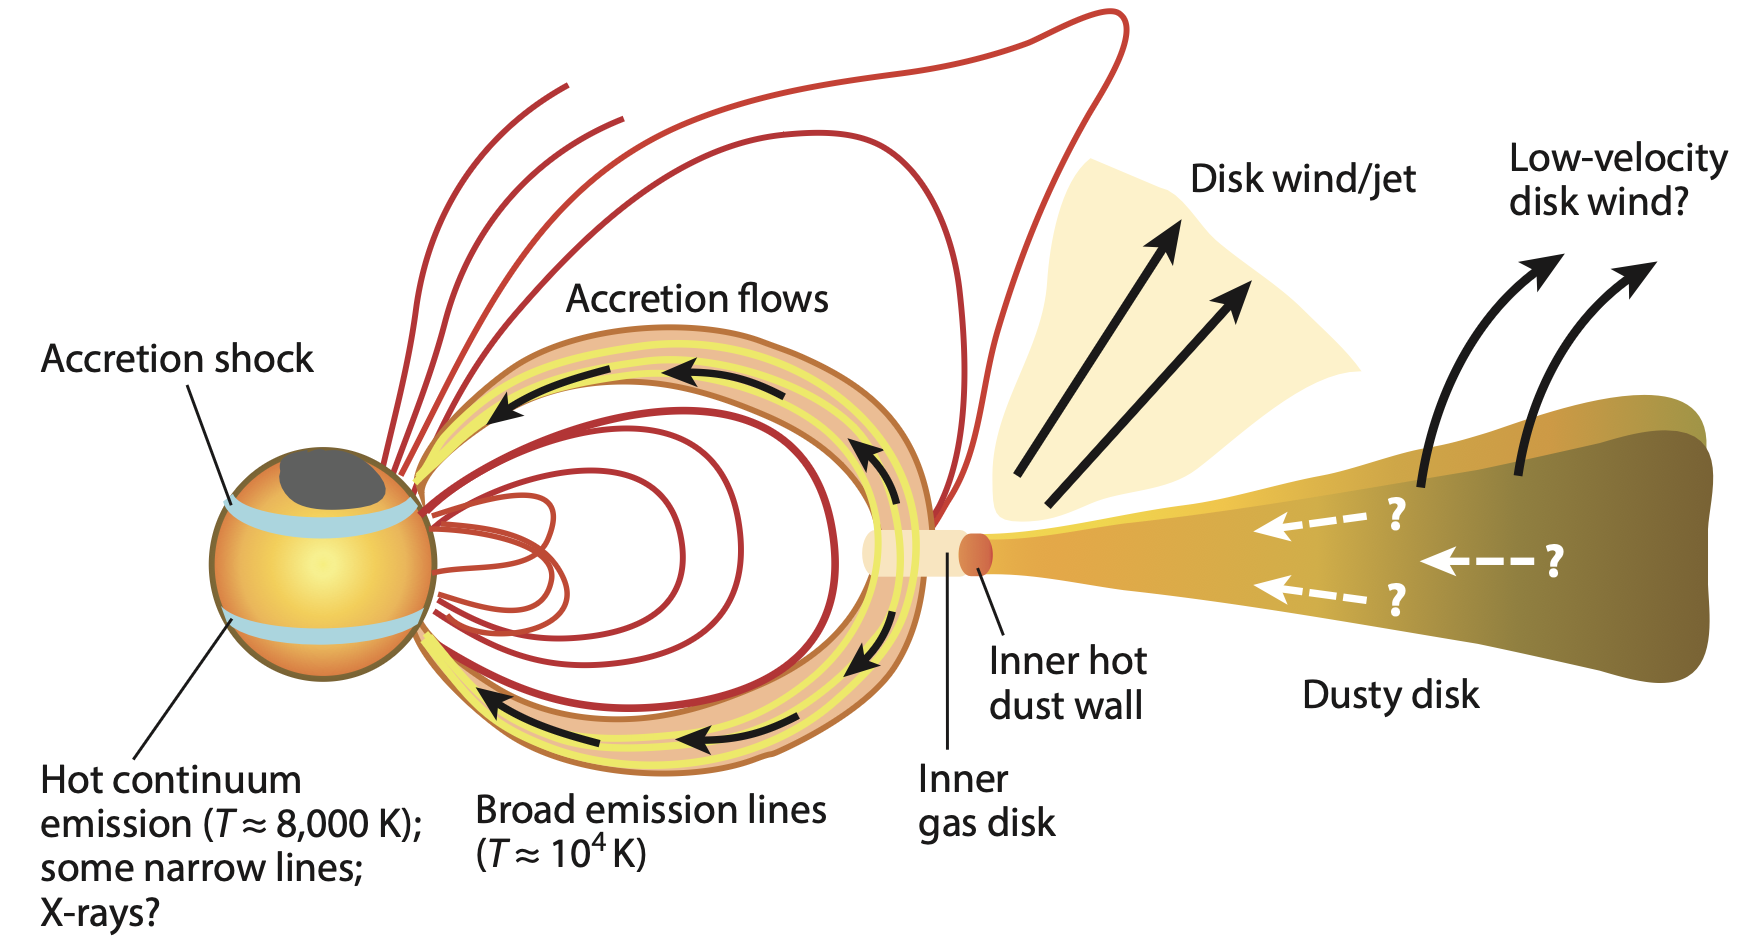
\includegraphics[width=.8\textwidth]{HartmannEtAl2016_magnetospheric_accretion.png}
  \caption{Schematic illustration of magnetospheric accretion onto young low-mass stars. The strong stellar magnetic field truncates the circumstellar disk at a few stellar radii. Accreting material is channeled along the magnetic field lines and impacts the stellar surface, forming an accretion shock. Jets and disk winds may also play a role in the star-disk interaction. The exact mechanisms for mass and angular momentum transport in the star-disk system remain uncertain. The figure is reproduced from Fig.~1 of \textcite{HartmannEtAl2016}.}
  \label{fig:magnetospheric_accretion}
\end{figure}

Stellar magnetic fields play a crucial role in the accretion of pre-main sequence stars, through the mechanism known as magnetospheric accretion \parencite[See, for example,][for a review]{HartmannEtAl2016}. Fig.~\ref{fig:magnetospheric_accretion} is a schematic illustration of magnetospheric accretion onto young ($1 \lesssim t \lesssim 10,\mr{Myr}$), low-mass ($\lesssim 1 M_\odot$) stars. The strong stellar magnetic field truncates the circumstellar disk at a few stellar radii. The dust disk is truncated slightly farther out than the gas disk, as dust in the inner disk sublimates due to heating by the stellar radiation field. The inner edge of the dust disk is responsible for most of the observed near-IR excess. Material from the disk is funneled onto the star along the magnetic field lines, where it is heated to approximately $10^4\,\mr{K}$, producing broad emission lines. The accretion flow is accelerated along the field lines, eventually reaching the stellar surface at nearly free-fall velocity. This process leads to the formation of an accretion shock at the stellar surface, where the gas is briefly halted and heated to very high temperatures, emitting X-rays. Most of these X-rays are absorbed and reradiated in the ultraviolet and optical continuum.

Despite recent advances in the study of magnetospheric accretion, many aspects are still under debate. \textcite{Bouvier2014} summarizes several open issues regarding the physics of the magnetospheric accretion and ejection processes. One of the long-standing problems is the evolution of stellar rotation: while the angular momentum carried by accreting material should spin up the star, observations reveal that the rotation rates of PMS stars are lower than expected. This discrepancy suggests that some form of magnetic braking must be at work to regulate stellar spin \parencite[e.g.,][]{HerbstEtAl2007}.

Magnetohydrodynamic simulations suggest that jets, disk winds, and magnetospheric ejections are involved in removing angular momentum during accretion \parencite[e.g.,][]{RomanovaEtAl2004,LiiEtAl2014,IrelandEtAl2020}. However, the relative importance of these mechanisms in shaping the angular momentum evolution remains under investigation \parencite[e.g.,][]{KunitomoEtAl2017}. Although the models presented in this work do not include magnetic fields or rotation, understanding the broader framework of magnetospheric accretion is essential for interpreting how accretion affects stellar structure. Including these physical processes for more realistic accretion modeling will be an important direction for future work.

\subsection{Observational evidence of magnetospheric accretion}
\label{sec:obs_evidence}

Observations of CTTSs provide strong evidence for magnetospheric accretion, including the presence of strong stellar magnetic fields, an inner cavity of a few stellar radii within the magnetosphere, magnetic accretion columns filled with free-falling plasma, and accretion shocks at the stellar surface.

The accretion shock produces emission in the ultraviolet, optical, and near-infrared wavelengths, as well as a modest amount of X-rays. These emissions serve as crucial diagnostics of the accretion region, allowing measurements of the accretion luminosity which, when combined with stellar mass and radius, provide estimates of accretion rates. Soft X-ray emission, unique to accreting stars, has also been detected from CTTSs and is likely produced in the post-shock region \parencite[e.g.,][]{KastnerEtAl2002}. Magnetospheric accretion flows can be identified by redshifted absorption features in specific spectral lines \parencite{MuzerolleEtAl2001}, while blueshifted forbidden emission lines have been linked to strong winds and mass outflows \parencite[e.g.,][]{Bally2016}.

% Accretion disks are commonly observed in star formation regions, and their presence is often inferred from the emission of infrared radiation from the dust in the disk. The accretion rate can be estimated from the luminosity of the accretion shock, which is typically observed in the ultraviolet and optical wavelengths. The accretion rate can also be estimated from the emission lines of hydrogen and other elements, which are often broadened by the Doppler effect due to the motion of the accreting material. There also have been direct images of the protoplanetary disks, the leftover of accretion disks, around young stars, such as the one taken by the Atacama Large Millimeter/submillimeter Array (ALMA).

Magnetospheric accretion paradigm assumes that the stellar magnetic field is strong enough to counteract the pressure of the accretion disk and disrupt the disk before it reaches the stellar surface \parencite[e.g.,][]{Koenigl1991}. At the truncation radius $R_\mr{trunc}$, the magnetic pressure approximately balances the gas ram pressure, i.e., $B^2/8\pi \simeq \frac{1}{2}\rho v^2$, where the relevant velocity is roughly the Keplerian velocity, $v = \sqrt{GM_\star/R_\mr{trunc}}$. The exact location of this truncation radius will also depend on the accretion rate \parencite[see Eq.~2.2 in][]{BouvierEtAl2007}. This framework generally aligns with the measured magnetic field strengths of CTTSs, which typically range from a few hundred Gauss to a few kiloGauss \parencite{BouvierEtAl2007,AlencarEtAl2012}. 

\section{Stellar evolution modeling}
\label{sec:stellar_evol}

Stellar evolution modeling involves combining physical principles with numerical methods to simulate how stars change over time. This section first introduces the fundamental equations that describe stellar evolution and then turns the focus to the modeling of pre-main sequence stars.

\subsection{Stellar structure equations}
\label{sec:stellar_evol_formulation}

Modeling stellar evolution involves defining initial conditions and solving the differential equations that govern the physical processes inside a star, thereby predicting how stellar properties change over time. The primary factors determining an isolated star's evolution are its mass and initial chemical composition. Once specified, these initial parameters are input into the stellar structure equations, which express the physical quantities as functions of position and time $(\vec{r}, t)$. By assuming spherical symmetry, the position can be reduced to the radial distance $r$ from the center, so physical quantities become functions of radius and time, i.e., $(r, t)$.

Throughout most of stellar evolution, the total stellar mass remains nearly constant except in cases of significant mass loss. In contrast, the stellar radius can vary rapidly as the star passes through different stages. Because Lagrangian coordinates move with the fluid elements, it is more convenient to use the mass coordinate $m$, defined as the total mass enclosed within radius $r$, rather than the radius itself. This approach allows us to track the evolution of specific mass shells as they move and change, making it a more natural choice for describing properties such as energy production, chemical composition and angular momentum within the stellar interior. 

In the mass coordinate, the system of 1D stellar structure equations can be written as \parencite[See, for example, ][]{KippenhahnEtAl2013}:
\begin{subequations}\label{eq:star_struct}
  \begin{align}
    % \pfird[p]{m} &= -\frac{G m}{4\pi r^2} + \frac{\Omega^2}{6 \pi r^2}, \label{eq:star_struct1}\\
    \pfird[p]{m} &= -\frac{G m}{4\pi r^2}, \label{eq:star_struct1}\\
    \pfird[T]{m} &= \pfird[p]{m} \frac{T}{p} \nabla, \label{eq:star_struct2}\\
    \pfird[r]{m} &= \frac{1}{4 \pi r^2 \rho}, \label{eq:star_struct3}\\
    \pfird[l]{m} &= \epsilon_\mr{nuc}  - \epsilon_\nu + \epsilon_\mr{g} , \label{eq:star_struct4}\\
    \pfird[X_i]{t} &= -\pfird[F_i]{m} + \Psi_i(p, T, \bvec{X}), 1\leq i \leq n_\mr{elem}, \label{eq:star_struct5}
  \end{align}
\end{subequations}
where $G$ is the gravitational constant, $\nabla \equiv \partial \ln T/\partial \ln p$ is the temperature gradient, $\rho$ is the density, and $\epsilon_\mr{nuc}$, $\epsilon_\nu$, and $\epsilon_\mr{g}$ are the rates of nuclear energy production, neutrino energy loss, and gravitational energy production, respectively, all expressed in units of power per unit mass. By definition, $\epsilon_\nu > 0$. $X_i$ is the abundance of the chemical element $i$, $F_i$ is the flux of the chemical element $i$ due to diffusion, $\bvec{X} \equiv \{X_i\}$ is the chemical composition vector, $\Psi_i$ is the rate of change of $X_i$ by thermonuclear reactions, and $n_\mr{elem}$ is the total number of chemical species considered. All quantities ($p, l, \rho, T, \epsilon, \epsilon_\nu$, etc.) are evaluated locally at each stellar layer.

Eq.~\eqref{eq:star_struct1} describes the hydrostatic equilibrium and Eq.~\eqref{eq:star_struct3} describes the mass continuity. Eq.~\eqref{eq:star_struct4} and Eq.~\eqref{eq:star_struct2} describe the energy production and energy transport, respectively. These equations illustrate a close coupling between stellar structure and the process of energy production and transport. In most stars, energy is primarily transported by radiation and convection, and the value of $\nabla$ depends on the dominant mechanism of energy transport. Eq.~\eqref{eq:star_struct5} describes the evolution of the chemical composition of the star, which is governed by the nuclear reactions occurring in the star and the transport of chemical elements. This set of equations assumes spherical symmetry and does not account for magnetic fields nor rotation. These are common simplifications in 1D stellar models and are sufficient for many evolutionary studies.

Stellar evolution is typically treated as a one-dimensional boundary value problem with initial conditions given by the initial mass and chemical composition of the star. The boundary conditions are set at the center and surface of the star. Spherical symmetry requires that the radius, luminosity, and chemical element fluxes vanish at the center of the star. Therefore, it is imposed that:
\begin{equation}
  r(0, t) = 0,\ l(0, t) = 0,\ F_i(0, t) = 0, i = 1, \ldots, n_\mr{elem}.
\end{equation}

At the surface, the pressure and temperature are set to the values at the base of the stellar atmosphere:
\begin{equation}
  p(M_\star, t) = p_\mr{atm}(L_\star, R_\star, t),\ T(M_\star, t) = T_\mr{atm}(L_\star, R_\star, t),
\end{equation}
where $M_\star$, $L_\star$, and $R_\star$ are the stellar mass, luminosity, and radius, respectively. The values of \(p_\mr{atm}\) and \(T_\mr{atm}\) are derived from reconstruction of the stellar atmosphere, which typically uses empirical relations. As this project focuses on internal structure, I will not delve into the specifics of atmospheric modeling.

With both central and surface boundary conditions specified, and the evolution equations defined in Lagrangian coordinates, the stellar structure problem becomes a well-posed initial-boundary value problem. This framework serves as the basis for numerical stellar evolution codes, which solve these equations to track the stellar evolution over time.

The solutions to the stellar structure equations yield key observable properties of stars, most notably their luminosity $L$ and effective surface temperature $T_\mr{eff}$. These two parameters define a star's position on the Hertzsprung-Russell (HR) diagram, a fundamental tool in astrophysics to understand and visualize stellar evolution. The HR diagram helps to reveal distinct evolutionary stages such as the pre-main sequence, main sequence, and giant branch, offering a simple way to compare models with observations.

However, translating the underlying physics into stellar models is a complex task. In practice, stellar evolution codes can differ substantially in their model initialization methods. These differences can lead to notable variations during the early evolutionary stages, which will be discussed in the Sec.~\ref{sec:pms_evolution}. Furthermore, differences in formulations, assumptions, and adopted physical ingredients, such as the equation of state (EoS) and opacities, can substantially influence the predicted stellar properties, often resulting in discrepancies between models. Therefore, it is essential to carefully consider the specific implementations and assumptions of each code when interpreting stellar evolution results. One of the goals of this project is to benchmark our accretion models against those implemented in other stellar evolution codes. The details of our physical inputs will be discussed in Sec.~\ref{sec:cesam2k20}. 

\subsection{Pre-main sequence evolution}
\label{sec:pms_evolution}

\subsubsection{Pre-main sequence evolution with constant mass}
\label{sec:pms_const_mass}

Classically, the modeling of PMS evolution begins with a fully convective star of large radius and luminosity. As the star contracts under gravity, the release of gravitational energy heats the stellar interior. This contraction continues until the central temperature becomes high enough to slow down the contraction and trigger the formation of a radiative core.

The initial phase of PMS evolution is characterized by a rapid decrease in both radius and luminosity, while the effective temperature remains nearly constant. This phase, known as the Hayashi track \parencite{Hayashi1961}, defines the locus in the HR diagram of fully convective stars of a given mass and composition. Energy transport is dominated by convection during this phase. The precise location and slope of the Hayashi track is also sensitive to the treatment of convection, typically modeled using the mixing-length theory \parencite{CoxGiuli1968a}. As the star contracts, its density increases, which in turn increases the opacity of the stellar material. The resulting decrease in radiative efficiency causes a reduction in luminosity. The Hayashi tracks appear on the far right of the HR diagram and follow a steep, nearly vertical path.

The Hayashi track terminates at a minimum luminosity, where the central temperature becomes high enough for hydrogen to be fully ionized. This leads to a substantial drop in opacity in the central regions, making radiative transport more efficient, and a radiative core forms. The star then evolves toward higher effective temperatures while its luminosity remains approximately constant. This marks the beginning of the second phase of PMS evolution, where the star follows a more horizontal path in the HR diagram, known as the Henyey track, first described by \textcite{HenyeyEtAl1955}. During this stage, the star evolves with a radiative core while maintaining a convective envelope.

This classic two-phase PMS evolution—first descending the vertical Hayashi track, then moving leftwards on the more horizontal Henyey track—is illustrated in Fig.~\ref{fig:hayashi_henyey_tracks}, which shows evolutionary tracks for \texttt{Cesam2k20} models with masses between $1$ and $5,M_\odot$, assuming initial composition $X \simeq 0.73$, $Y \simeq 0.25$ (see Sec.\ref{sec:cesam2k20} for details of the input physics). Arrows indicate the direction of stellar evolution, with mass labels marking the ends of each track. The nearly vertical portion corresponds to fully convective contraction (Hayashi track), while the more horizontal portion marks the emergence of a radiative core (Henyey track)..

During PMS evolution, gravitational contraction remains the primary energy source, as the central temperature has not yet reached the threshold for hydrogen fusion. However, light elements such as deuterium and lithium can be burned at relatively low temperatures \parencite{KippenhahnEtAl2013}.

Deuterium burning is particularly important in PMS evolution, proceeding via the reaction:
\begin{equation}
  ^2\mr{H} + ^1\mr{H} \rightarrow ^3\mr{He} + \gamma,\quad \Delta E_\mr{D} = 5.5\,\mr{MeV},
\end{equation}
which ignites at central temperature of $T_c \sim 10^6,\mr{K}$. 

Lithium burning, involving the dominant isotope $^7$Li, occurs via the reaction:
\begin{equation}
  ^7\mr{Li} + ^1\mr{H} \rightarrow ^4\mr{He} + ^4\mr{He} + \gamma,\quad \Delta E_\mr{Li} = 17.6\,\mr{MeV},
\end{equation}
which sets in at $T_c \sim 2.5 \times 10^6,\mr{K}$. Although lithium burning releases significantly more energy per reaction than deuterium burning, the former makes little contribution to the total energy production in PMS stars, as lithium is around $10^3$ less abundant than deuterium \parencite{GrevesseSauval1998}.

\begin{figure}[htbp]
  \centering
  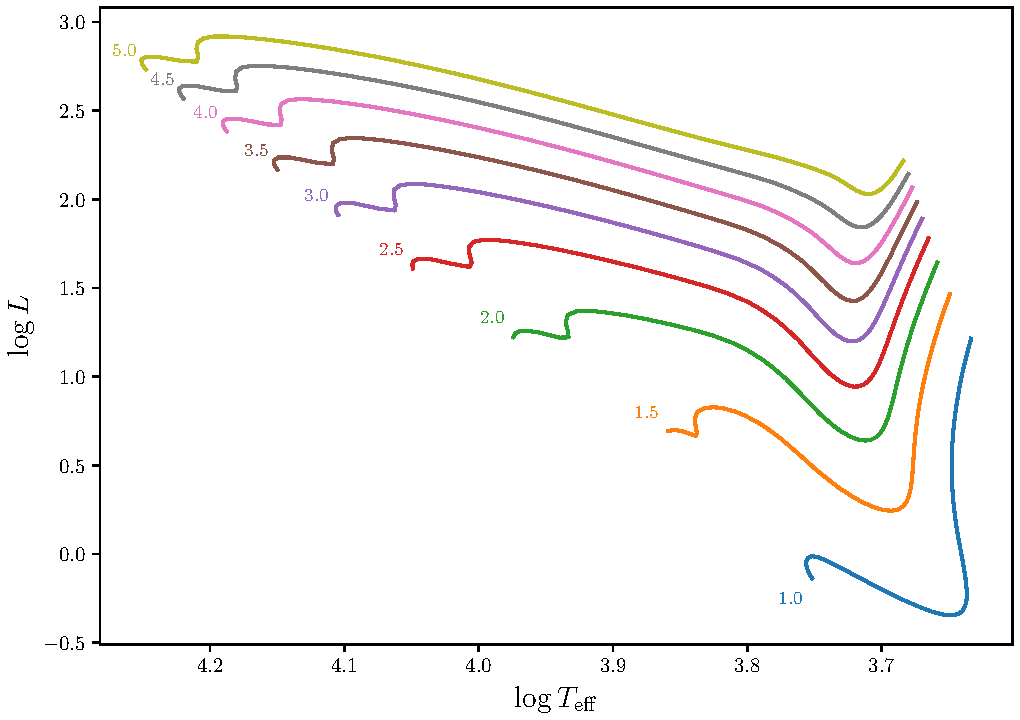
\includegraphics[width=.75\textwidth]{classic_pms.pdf}
  \caption{Classic pre-main sequence evolutionary tracks for \texttt{Cesam2k20} models with masses between $1$ and $5,M_\odot$ in the HR diagram. Arrows indicate the direction of stellar evolution, with stellar masses in solar masses labeled at the end of each track. The nearly vertical Hayashi track corresponds to fully convective contraction, while the more horizontal Henyey track marks the phase when contraction slows down and a radiative core develops.} \label{fig:hayashi_henyey_tracks}
\end{figure}

The star is considered to have reached the main sequence once hydrogen fusion becomes the dominant source of energy production, at a central temperature of $T_c \sim 10^7\,\mr{K}$. This beginning of main sequence evolution is referred to as the Zero-Age Main Sequence (ZAMS). From the ZAMS onward, the star's position in the HR diagram changes relatively slowly during the long phase of central hydrogen burning.

\subsubsection{Pre-main sequence evolution with accretion}
\label{sec:pms_accretion}

The classic PMS evolution described above assumes that the star has already acquired its final mass at the beginning of contraction. However, as the observational evidence discussed in Sec.~\ref{sec:obs_evidence} indicates, many young stars continue to accrete material from their surrounding environment during the PMS phase. These stars experience a period of relaxation and thermal re-adjustment as they contract, before eventually settling onto a track that closely follows the constant-mass evolution \parencite{KippenhahnEtAl2013}.

One physical quantity of importance in this context is the mass accretion rate $\dot{M}_\mr{acc}$,  defined as the rate at which mass is transferred from the surrounding cloud to the protostar. Estimates of $\dot{M}_\mr{acc}$ are often uncertain by factors of a few, due to their sensitivity to stellar parameters and extinction. These values are typically calculated from the accretion luminosity $L_\mr{acc}$ via:
\begin{equation}
  L_\mr{acc} = \frac{GM_\star \dot{M}_\mr{acc}}{R_\star}\left(1 - \frac{R_\star}{R_\mr{trunc}}\right),
\end{equation}
assuming the material falls freely from the truncation radius $R_\mr{trunc}$ to the stellar surface at radius $R_\star$, \parencite[see review by][]{HartmannEtAl2016}. 

\begin{figure}[htbp]
  \centering
  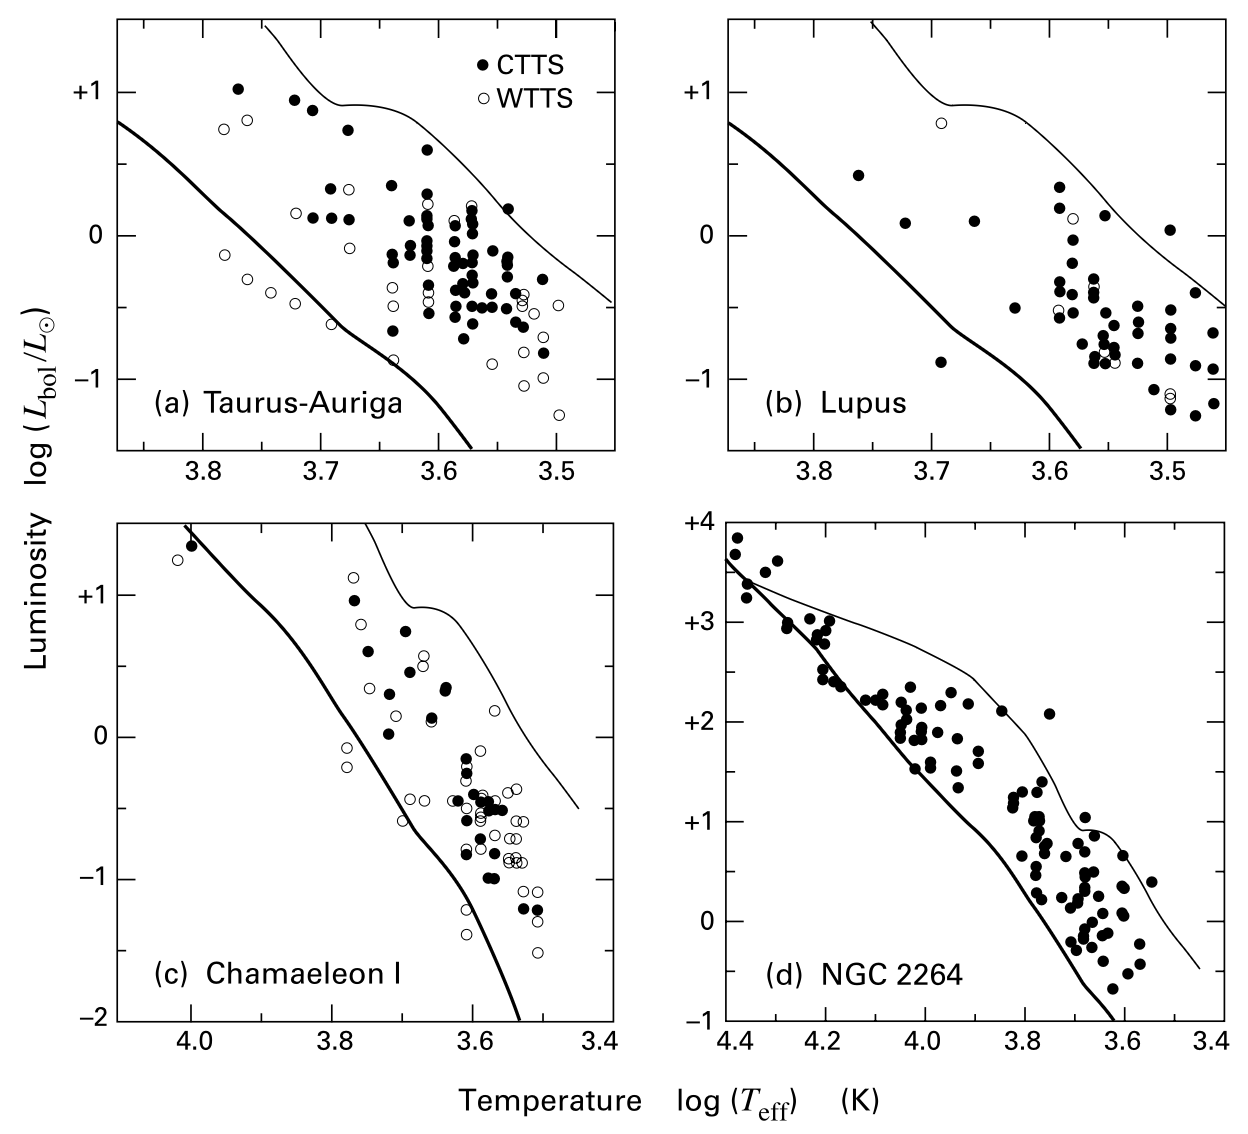
\includegraphics[width=.85\textwidth]{StahlerPalla2004_fig4p9.png}
  \caption{HR diagrams for four stellar associations. In panels (a)-(c), closed circles represent CTTSs, while open circles are WTTSs. In panel (d), the sample includes CTTSs, Herbig Ae/Be stars, and main sequence objects. The thin upper curves are the theoretical birthlines; the thick lower curves are the ZAMS. Reproduced from Fig.~4.9 of \textcite{StahlerPalla2004}.} \label{fig:obs_birthline} 
\end{figure}

Observational studies reveal a correlation between accretion rates and stellar mass, with more massive stars accreting at higher rates \parencite[e.g.,][]{MuzerolleEtAl2003,ManaraEtAl2017,RugelEtAl2018,LanzafameEtAl2023}. Models of viscous disk evolution predict a declining $\dot{M}_\mr{acc}$ with stellar age as the circumstellar disk becomes depleted \parencite[e.g.,][]{HartmannEtAl1998,GortiHollenbach2009}.  Despite this, the precise functional form of the mass and time dependence remains under debate. For this study, a constant accretion rate $\dot{M}_\mr{acc}$ is adopted for simplicity.

Deuterium plays a more prominent role in accreting PMS stars than in non-accreting ones, as the accretion flow continuously supplies fresh deuterium. In contrast, non-accreting stars can deplete their initial deuterium rapidly. This deuterium contributes to energy generation through nuclear burning at a rate given by
\begin{equation}
  \epsilon_\mr{D} = \left[\mr{D/H}\right]\epsilon_\mr{D,0} \left(\frac{\rho}{1,\mr{g,cm^{-3}}}\right) \left(\frac{T}{1 \times 10^6,\mr{K}}\right)^{n_D}, \label{eq:deuterium_energy_prod_rate}
\end{equation}
where $\epsilon_\mr{D,0} = 4.19 \times 10^7,\mr{erg,g^{-1},s^{-1}}$, $n_D = 11.8$, and $\left[\mr{D/H}\right]$ is the number density of deuterium relative to hydrogen in the environment \parencite[cf. Eq.~11.27 in][]{StahlerPalla2004}.

The amount of deuterium in the accreted material can strongly influence PMS evolution. High deuterium abundance leads to significant stellar expansion during accretion, while low abundance results in a smaller size of the star throughout evolution toward the main sequence \parencite{KunitomoEtAl2017}.

When the main accretion phase ends, the circumstellar disk has mostly been dissipated and become optically thin, allowing the star to appear as a visible object. The locus in the HR diagram where PMS stars of different masses first become visible is known as the birthline \parencite{Stahler1983}. Its position is sensitive to the star's accretion history, initial mass, and chemical composition.

Theoretical birthlines can be compared with observations of TTSs to evaluate models of PMS evolution. Moreover, the birthline provides insights into the environments in which stars are formed. In Fig.~\ref{fig:obs_birthline}, observations of four stellar associations with active star formation are plotted alongside the theoretical birthline and the ZAMS. Stars located below the birthline have recently dispersed their circumstellar envelopes, whereas younger, still-embedded stars cannot yet be placed on the HR diagram due to difficulties in measuring their effective temperatures.

\section{Methods}
\label{sec:methods}

\subsection{The consequences of accretion}
\label{sec:accretion_modeling}

The most direct consequence of accretion onto a star is the increase in its mass. However, accretion also alters the stellar environment and affects the star's radiative output by delivering additional energy. It can also supply fresh deuterium, which contributes significantly to the star's energy budget through nuclear burning.

As discussed in Sec.~\ref{sec:magnetospheric_accretion}, accretion is a highly complex process involving various physical mechanisms, such as angular momentum transport from the disk to the star, magnetic fields, and outflows like jets and winds. To make the problem tractable in the context of stellar evolution, some simplifications are necessary. In this section, I describe how the consequences of accretion are incorporated into stellar evolution models, focusing on the treatment of gravitational energy, deuterium from accreted material, and the regimes of hot and cold accretion.

Before moving into more details, it is important to note that gravitational energy associated with accretion comes from two distinct sources:
\begin{enumerate}
  \item The gravitational energy released (or absorbed) by the star due to contraction or expansion during its evolution, and
	\item The gravitational potential energy of the material as it falls onto the star, which is partly converted into the thermal energy of the accreted material before it reaches the stellar surface.
\end{enumerate}

The former affects the internal energy budget of the star itself, while the latter relates to how the infalling material delivers its energy upon impact, which depends on the nature of the accretion process (see Sec.~\ref{sec:hot_cold_accretion}).

\subsubsection{Gravitational energy}
\label{sec:grav_energy}

The gravitational energy released during the PMS phase contributes significantly to the stellar energy budget and must be properly accounted for in stellar evolution models. In this section, I describe how this energy is treated in the stellar structure equations, and in the following section, I discuss the specific treatment of gravitational energy associated with accreted material.

The rate of gravitational energy release per unit mass is gievn by:
\begin{equation}
\epsilon_g = -T\left.\pfird[s]{t}\right|_m, \label{eq:grav_energy}
\end{equation}
where $s$ is the specific entropy.

From the first law of thermodynamics, $\dd{q} = \dd{u} + p\dd{v}$, where $u$ is the specific internal energy and $v = 1/\rho$ is the specific volume, one can write:
\begin{equation}
  T\left.\pfird[s]{t}\right|_m = \pfird[q]{t} = \pfird[u]{t} + p\pfird[v]{t} = \pfird[u]{t} - \frac{p}{\rho^2}\pfird[\rho]{t}.
\end{equation}

In practice, the internal energy depends on the chemical composition and the equation of state, which complicates the calculation. However, for a chemically homogeneous star, we can use the Kippenhahn approximation \parencite{KippenhahnEtAl2013}, which instead expresses the entropy change as:
\begin{equation}
  T\left.\pfird[s]{t}\right|_m \simeq c_p\pfird[T]{t} - \frac{\delta}{\rho}\pfird[p]{t},
\end{equation}
where $c_p$ is the specific heat at constant pressure and $\delta = -\left(\partial \ln \rho / \partial \ln T\right)_p$. 

Since PMS stars are generally fully convective, chemical mixing is highly efficient throughout the interior, which makes the Kippenhahn approximation appropriate in this context of this project.

With this, Eq.~\eqref{eq:star_struct4} becomes:
\begin{equation}
  \pfird[l]{m} = \epsilon_\mr{nuc} - \epsilon_\nu - c_p\pfird[T]{t} + \frac{\delta}{\rho}\pfird[p]{t}. \label{eq:grav_energy_kipp}
\end{equation}

However, applying Eq.~\eqref{eq:grav_energy_kipp} to evolving stellar models with accretion presents a complication: the thermodynamic and chemical properties of the accreted material are not provided directly by the stellar model. Estimating these properties requires special treatment, which is addressed in the next two sections.

\subsubsection{Coordinate transformation for accretion modeling}
\label{sec:accretion_coords}

To incorporate accreted mass into the stellar model, its thermal and compositional properties must be specified. A common simplification for the thermal structure is to assume that the accreted material is homologous to the stellar surface—that is, it shares the same entropy. This assumption is justified by comparing characteristic timescales. The thermal timescale of a mass element, $\tau_\mathrm{th} \simeq \Delta m, c_p T / L$, describes how quickly it reaches thermal equilibrium with its surroundings. The accretion timescale, $\tau_\mathrm{acc} \simeq \Delta m / \dot{M}\mathrm{acc}$, is the time over which the mass is accreted. When $\tau\mathrm{th} \ll \tau_\mathrm{acc}$, the accreted material has time to thermally equilibrate with the stellar surface,  thereby justifying the use of the homologous assumption. This condition is equivalent to $\dot{M}_\mathrm{acc} c_p T \ll L$, which is typically satisfied near the stellar surface \parencite{SugimotoNomoto1975,PaxtonEtAl2015}. 

This assumption permits the use of fractional mass coordinates, defined as \parencite{SugimotoNomoto1975}
\begin{equation}
  q_m = \frac{m}{M_\star}.
\end{equation}

Switching from the Lagrangian mass coordinate $m$ to the fractional mass coordinate $q_m$ modifies the form of time derivatives in the structure equations. For a generic function $f(m,t)$, the total differential can be expressed both in terms of $m$ and $q_m$:
\begin{align}
  \dd{f} &= \left.\pfird[f]{t}\right|_{q_m} \dd{t} + \left.\pfird[f]{q_m}\right|_t\dd{q_m}\\ 
  &= \left.\pfird[f]{t}\right|_{q_m} \dd{t} + \left.\pfird[f]{q_m}\right|_t\left(\left.\pfird[q_m]{t}\right|_m \dd{t} + \left.\pfird[q_m]{m}\right|_t \dd{m}\right)\\
  \dd{f} &= \left.\pfird[f]{t}\right|_m \dd{t} + \left.\pfird[f]{m}\right|_t \dd{m}
\end{align}

Equating the two expressions yields:
\begin{equation}
  \left.\pfird[f]{t}\right|_m = \left.\pfird[f]{t}\right|_{q_m} + \left.\pfird[f]{q_m}\right|_t \left.\pfird[q_m]{t}\right|_m
  % &\left.\pfird[f]{m}\right|_t = \left.\pfird[f]{q_m}\right|_t\left.\pfird[q_m]{m}\right|_t.
\end{equation}

Using this, Eq.~\eqref{eq:grav_energy} can be rewritten in terms of $q_m$ as:
\begin{equation}
   \epsilon_g = -T \left.\pfird[s]{t}\right|_{q_m} - T \left.\pfird[s]{q_m}\right|_t\left.\pfird[q_m]{t}\right|_m.
\end{equation}
While the expressions for $\epsilon_g$ in Eq.~\eqref{eq:grav_energy} and its reformulation above are physically equivalent, the latter is more convenient when the time derivative at fixed mass coordinate is not readily available.

\subsubsection{Deuterium from the accreted material}
\label{sec:deuterium_burning}

In contrast to the thermal properties, the chemical composition of the accreted material is not necessarily homologous to that of the stellar surface. In particular, the deuterium content of the accreted gas can differ significantly from that of the star. This difference arises because deuterium burning becomes extremely efficient once the central temperature exceeds a critical threshold. Since PMS stars are generally fully convective, efficient mixing ensures that the entire interior remains chemically homogeneous. As a result, deuterium can be depleted as fast as it is supplied, leaving the stellar interior nearly devoid of it, even while fresh deuterium continues to arrive from the surrounding environment.

The amount of deuterium in the accreted material can significantly affect the evolution of PMS stars \parencite[e.g.,][]{KunitomoEtAl2017,AmardMatt2023}. Deuterium burning provides a substantial amount of energy that can halt or even reverse the star's contraction, thereby influencing both its radius and luminosity. In this sense, deuterium acts as a thermostat: because the nuclear energy generation rate $\epsilon_\mr{D}$ is highly sensitive to temperature (as seen in the exponent $n_\mr{D} = 11.8$ in Eq.~\eqref{eq:deuterium_energy_prod_rate}), a rise in central temperature dramatically increases $\epsilon_\mr{D}$, causing the star to expand. This expansion reduces the central temperature, which in turn suppresses the burning rate \parencite{StahlerPalla2004}—a self-regulating feedback mechanism.

This thermostatic behavior can only be sustained if deuterium is replenished at a sufficient rate. At steady-state burning, the deuterium luminosity can be approximated as:
\begin{equation}
  L_\mr{D} \equiv \int_0^{M_\star} \epsilon_\mr{D}\dd{m} \simeq \dot{M}_\mr{acc} \delta,
\end{equation}
where $\delta$ is the energy available from deuterium per gram of accreted material:
\begin{equation}
  \delta = \frac{[\mr{D/H}]X\Delta E_\mr{D}}{m_\mr{H}}.
\end{equation}
Here, $X \sim 0.73$ is the hydrogen mass fraction, $\Delta E_\mr{D} = 5.5\,\mr{MeV}$ is the energy released per deuterium fusion reaction, and $m_\mr{H}$ is the mass of a hydrogen atom.

The deuterium-to-hydrogen ratio, $[\mr{D/H}]$, in the accreted material is typically assumed to match that of the interstellar medium (ISM). However, its precise value remains uncertain. Observations of the local ISM suggest a wide range of values, from $0.98 \pm 0.38 \times 10^{-5}$ \parencite{HebrardEtAl2005} to at least $2.13 \pm 0.24 \times 10^{-5}$ \parencite{LinskyEtAl2006}. Moreover, $[\mr{D/H}]_\mr{ISM}$ is expected to evolve over time, since estimates of the primordial deuterium abundance, $[\mr{D/H}]_\mr{prim} \sim 2.5 \times 10^{-5}$, are higher than those observed in the local ISM \parencite[e.g.,][]{Prantzos2007}. As shown by \textcite{KunitomoGuillot2021}, the deuterium content in the accretion disk may also evolve over time due to the formation and growth of planetesimals, further complicating the picture.

Due to these complications, in this study I do not account for the time evolution of $[\mr{D}/\mr{H}]$. Instead, I adopt a fixed value of $[\mr{D}/\mr{H}] = 2.0 \times 10^{-5}$ for the accreting models and explore variations in this parameter to assess its impact on the evolution of PMS stars.

\subsubsection{Hot and cold accretion}
\label{sec:hot_cold_accretion}

As material accretes onto a PMS star, it brings gravitational potential energy and possibly some internal (thermal) energy. How much of this energy is deposited into the star depends strongly on the nature of the accretion process. Two main factors influence the efficiency of energy deposition:
\begin{enumerate}
  \item the geometry of the accretion flow (e.g., spherical or disk-like), and
  \item the radiative losses at the accretion shock and the stellar surface.
\end{enumerate}

Regarding the accretion geometry, each unit mass of accreted gas carries a gravitational potential energy of $-GM_\star/R_\star$ and internal energy $\beta GM_\star/R_\star$. The factor $\beta$ characterizes the physical nature of the accretion flow. For example, for gravitationally bound material, $\beta \leq 1$, while for thin-disk accretion from the equatorial region, typical values are $\beta \leq 0.5$ \parencite{PrialnikLivio1985,HartmannEtAl1998}.

The fractional surface area covered by accretion shock can influence the radiative efficiency, as the shocked region and the stellar photosphere have different radiative properties. Let $f_\mr{shock}$ denote the fraction of the stellar surface covered by the shock. The shocked area emits an accretion luminosity $L_\mr{acc} = 4\pi R_\star^2 f_\mr{shock} F_\mr{acc}$, where $F_\mr{acc}$ is the mean radiative flux over the accreting region. Meanwhile, the remaining stellar surface radiates at the star's intrinsic luminosity, $L_\mr{photo} = 4 \pi R_\star^2 (1 - f_\mr{shock}) T_\mr{eff}^4$. The total losses from the shock and the photosphere counteract the energy injection from the accreted material.

Following the simplified treatment by \textcite{HartmannEtAl1998}, these considerations can be combined into an effective energy injection rate from the accreted material:
\begin{equation}
  L_\mr{add} = \xi_\mr{add}\frac{GM_\star \dot{M}}{R_\star},
\end{equation}
where $\xi_\mr{add}$\footnote{My $\xi_\mr{add}$ is equivalent to $\alpha$ in \textcite[Eq.~(5)][]{HartmannEtAl1998}.} is a dimensionless parameter to quantity the fraction of accretion energy converted injected into the star. The value of $\xi_\mr{add}$ depends on both factors mentioned above. Radiative transfer calculations by \textcite{StahlerEtAl1980} show that $\xi_\mr{add} \leq 3/4$, while for disk accretion the upper limit is typically $\xi_\mr{add} \simeq 0.5$. This value can be further reduced by stellar rotation, which converts some of the accretion energy into angular momentum \parencite{KunitomoEtAl2017}. The case of $\xi_\mr{add} = 0.5$ is referred to as hot accretion, while $\xi_\mr{add} = 0$ is referred to  as cold accretion, as in this case no heat is injected into the stellar interior.

This heat injection can affect the evolution of accreting stars \parencite[e.g., ][]{KunitomoEtAl2017,AmardMatt2023}. However, for simplicity, heat injection during accretion is not included in this work. By neglecting this effect, I am effectively considering the case where $\xi_\mr{add} = 0$, which is a reasonable approximation for most PMS stars, as the majority of the accretion energy is expected to be radiated away before reaching the star \parencite{HartmannEtAl1998}.

\subsection{The stellar evolution code \texttt{Cesam2k20}}
\label{sec:cesam2k20}

We use the stellar evolution code \texttt{Cesam2k20} \parencite{MarquesEtAl2013,MorelLebreton2008,Morel1997} to model stellar evolution with accretion. \texttt{Cesam2k20} is an open-source, one-dimensional stellar evolution code (available at the \href{https://www.ias.u-psud.fr/cesam2k20/home.html}{Cesam2k20 website}) that employs a spectral method to solve the stellar structure equations given in Eqns.~\eqref{eq:star_struct}. To our knowledge, it is the only stellar evolution code that utilizes a spectral method, which offers the advantages of superconvergence and high numerical precision compared to the more commonly used finite-difference methods in stellar evolution modeling. The following subsections describe its numerical implementation, including the choice of variables, automatic grid-point allocation, the formulation of the structure equations, and the adopted input physics.

\subsubsection{Lagrangian variables}
\label{sec:cesam2k20_variables}

The system of equations in Eqns.~\eqref{eq:star_struct} encapsulates the fundamental physics governing stellar structure and evolution. However, in numerical implementation, these equations are often reformulated to improve stability and convergence. One effective approach, discussed by \textcite{Morel1997}, is to use the set of variables introduced by \textcite{Eggleton1971},
\begin{equation*}
\left(\frac{m}{M_\odot}\right)^{2/3},\quad \left(\frac{r}{R_\odot}\right)^2,\quad \left(\frac{l}{L_\odot}\right)^{2/3}, \quad l \geq 0
\end{equation*}
This choice improves numerical precision and helps avoid singularities at the stellar center. In cases where $l < 0$—which can occur during late evolutionary stages—the variable $l/L_\odot$ is used instead. Since this project focuses on the pre-main sequence phase, where such cases do not arise, we adopt the Eggleton variables throughout.

Additionally, because pressure and temperature can span several orders of magnitude in the stellar interior, it is numerically advantageous to work with their logarithms. Accordingly, the set of variables ultimately used in \texttt{Cesam2k20} is:
\begin{equation}
\xi = \ln P,\quad \eta = \ln T,\quad \zeta = \left(\frac{r}{R_\odot}\right)^2,\quad \lambda = \left(\frac{l}{L_\odot}\right)^{2/3},\quad \mu = \left(\frac{m}{M_\odot}\right)^{2/3}.
\end{equation}

\subsubsection{Automatic location of grid points}
\label{sec:cesam2k20_grid}

To resolve the large variations in physical quantities during stellar evolution, an adaptive grid is necessary. To achieve automatic allocation, \texttt{Cesam2k20} uses a strictly monotonic spacing function, $Q(\mu, t)$, to distribute grid points based on local physical conditions. Grid points are placed such that the difference in $Q(\mu, t)$ between adjacent points is equal to a time-dependent spacing function $\psi(t)$ \parencite{Eggleton1971,PressEtAl1992,Morel1997}.

Formally, at each time step $t$, the grid points $\mu_i,\ i = 1,\ldots,n$ are allocated such that:
\begin{equation}
  Q(\mu_{i+1}, t) - Q(\mu_i, t) = \psi(t),\quad i = 1, \ldots, n-1,
\end{equation}
where $\psi(t)$ is determined during the numerical integration. 

The default form of the spacing function $Q(\mu, t)$ used in \texttt{Cesam2k20} is:
\begin{equation}
  % Q(\mu, t) = -\xi + 15\mu. \label{eq:cesam2k20_spacing_func}
  Q(\mu, t) = (-1)\xi + (0)\eta + (0)\zeta + (0)\lambda + (15)\mu, \label{eq:cesam2k20_spacing_func}
\end{equation}
where the values in parentheses serve as weights for each variable in the calculation of the distance between grid points. See \textcite{Morel1997,Manchon2021} for the rationale behind this choice. These coefficients can be adjusted in the numerical settings to achieve higher resolution in specific variables if desired. The dependence of $Q(\mu, t)$ on pressure ($\xi$) and mass ($\mu$) ensures finer resolution in regions of steep pressure and density gradients. In the core, where the pressure gradient is modest, resolution is primarily controlled by mass change; while in the outer envelope, where pressure varies rapidly, the grid is refined mostly based on pressure changes.

To map physical coordinates onto the numerical grid, \texttt{Cesam2k20} defines an index function $q(\mu, t)$ that takes integer values from $1$ to $n$ at the grid points. Values of physical variables at positions between grid points are obtained by interpolation on the grid. The derivative of $Q$ with respect to this index gives:
\begin{equation}
  \left.\pfird[Q]{q}\right|_t = \left.\pfird[Q]{\mu}\right|_t\left.\pfird[\mu]{q}\right|_t = \theta(\mu, t)\left.\pfird[\mu]{q}\right|_t = \psi(t),
\end{equation}
where $\theta(\mu, t)$ is directly obtained from the analytic form of $Q(\mu, t)$ in Eq.~\eqref{eq:cesam2k20_spacing_func}.

The introduction of $\psi(t)$ and $\theta(\mu, t)$ requires two additional equations for closure:
\begin{equation}
  \pfird[\mu]{q} = \frac{\psi}{\theta},\quad \pfird[\psi]{q} = 0.
\end{equation}
The first equation relates the mass coordinate to grid index, while the second enforces constant spacing in $Q$-space. This approach enables efficient resolution of the stellar structure, especially during rapid evolutionary phases.

\subsubsection{Structure equations}
\label{sec:cesam2k20_struct_eq}

With the variables introduced in Secs.~\ref{sec:cesam2k20_variables} and \ref{sec:cesam2k20_grid}, the stellar structure equations can be expressed in a form more suitable for integration on an equidistant grid in the numerical index $q_i = 1, \ldots, n$. 

The full set of structure and composition equations solved at each time step is:
\begin{subequations} \label{eq:cesam2k20_struct_eq}
  \begin{align}
    0 &= \pfird[\xi]{q} - \left[-\frac{3G}{8\pi}\left(\frac{M_\odot}{R_\odot}\right)^2\left(\frac{\mu}{\zeta}\right)^2 + \frac{M_\odot}{4\pi R_\odot}\left(\frac{\mu}{\zeta}\right)^{1/2} \Omega^2\right]e^{-\xi}\frac{\psi}{\theta}, \label{eq:cesam_struct1}\\
    0 &= \pfird[\eta]{q} - \left[-\frac{3G}{8\pi}\left(\frac{M_\odot}{R_\odot}\right)^2\left(\frac{\mu}{\zeta}\right)^2 + \frac{M_\odot}{4\pi R_\odot}\left(\frac{\mu}{\zeta}\right)^{1/2} \Omega^2\right]e^{-\xi}\frac{\psi}{\theta}\nabla, \label{eq:cesam_struct2}\\
    0 &= \pfird[\zeta]{q} - \frac{3}{4\pi}\frac{M_\odot}{R_\odot^3}\frac{1}{\rho}\left(\frac{\mu}{\zeta}\right)^{1/2}\frac{\psi}{\theta}, \label{eq:cesam_struct3}\\
    0 &= \pfird[\lambda]{q} - \frac{M_\odot}{L_\odot}\left(\frac{\mu}{\lambda}\right)^{1/2}(\epsilon  + \epsilon_\nu + \epsilon_\mr{g})\frac{\psi}{\theta}, \label{eq:cesam_struct4}\\
    0 &= \pfird[\mu]{q} - \frac{\psi}{\theta}, \label{eq:cesam_struct5}\\
    0 &= \pfird[\psi]{q}, \label{eq:cesam_struct6}\\
    0 &= \pfird[X_i]{t} + \frac{2}{3 M_\odot\mu^{1/2}}\pfird[F_i]{\mu} - \Psi_i(\xi, \eta, \bvec{X}), 1\leq i \leq n_\mr{elem}. \label{eq:cesam_struct7}
  \end{align}
\end{subequations}

These equations are solved simultaneously with boundary conditions-at the center:
\begin{equation}
  \zeta(1, t) = 0,\quad \lambda(1, t) =0, \quad \mu(1, t) = 0,
\end{equation}
and at the surface:
\begin{equation}
  \xi(n, t) = \xi_\mr{atm}(L_\star, R_\star, t),\quad \eta(n, t) = \eta_\mr{atm}(L_\star, R_\star, t),\quad \mu(n, t) = \mu_\mr{atm},
\end{equation}
along with constitutive relations (e.g., equations of state, opacity laws) to evolve the stellar model in time.

\subsubsection{Input physics}
\label{sec:cesam2k20_input_physics}

Although \texttt{Cesam2k20} is capable of modeling rotation and diffusion, I keep the input physics simple at this stage to focus on the impact of accretion on stellar structure. The interactions of accretion with rotation and diffusion will be an important aspect in future work. The models are computed for 1D, single stars without rotation, magnetic fields, or diffusion. Mass loss is not considered; the only mechanism that alters the stellar mass is accretion. The initial chemical composition follows the solar mixture of \textcite{AsplundEtAl2009}, with meteoritic determination for non-volatile elements as recommended by \textcite{SerenelliEtAl2009}, with the exception of the deuterium abundance, which is varied to explore its impact on accreting stars.

Convection is modeled using the mixing-length theory (MLT) \parencite{CoxGiuli1968a}. It assumes that convective energy transport occurs via fluid elements moving from hotter to cooler regions over a characteristic distance-the mixing length—typically taken to be proportional to the pressure scale height. This proportionality is set by the mixing-length parameter, $\alpha_\mr{MLT}$. We adopt a solar-calibrated value of $\alpha_\mr{MLT} = 1.64$. Convective boundaries are determined using the Schwarzschild criterion, with no convective overshooting.

The equation of state (EoS) and opacity are interpolated from the OPAL2005 tables \parencite{RogersIglesias1992,IglesiasRogers1996,RogersNayfonov2002}, and supplemented at low temperatures by the AF opacity tables \parencite{FergusonEtAl2005}. Nuclear reaction rates are based on NACRE \parencite{AikawaEtAl2006} and LUNA \parencite{BrogginiEtAl2018} tables. The models include the full PP and CNO cycles, tracking the evolution of abundances for $^{1}\mr{H}$, $^{2}\mr{H}$, $^{3}\mr{He}$, $^{4}\mr{He}$, $^{7}\mr{Li}$, $^{7}\mr{Be}$, $^{12}\mr{C}$, $^{13}\mr{C}$, $^{14}\mr{N}$, $^{15}\mr{N}$, $^{16}\mr{O}$, $^{17}\mr{O}$.

Neutrino energy losses are treated using the prescriptions of \textcite{HaftEtAl1994} for plasma neutrinos and \textcite{Weigert1966} for photoneutrinos. The atmosphere is implemented using a Hopf $T(\tau)$ relation from \textcite{HubenyMihalas2015}, with the base of the atmosphere set at an optical depth of $\tau_{\max} = 20$, where the solution of the internal structure equations is matched to that of the atmosphere model.

\begin{table}
    \hfill
    \begin{tabularx}{.8\textwidth}{|| c | c ||}
        \cline{1-2}
        Parameter Type & Description \\ \cline{1-2}\\[-1em]\cline{1-2}
        Mass & accretion + no mass loss\\ \cline{1-2}
        Chemical composition  & AGS09+S10\footnotemark[1]\\ \cline{1-2}
        Convection & MLT\footnotemark[2] + No overshoot\\ \cline{1-2}
        Diffusion & None \\ \cline{1-2}
        EoS & OPAL2005\footnotemark[3] \\ \cline{1-2}
        Opacity & OPAL and AF \footnotemark[4]\\ \cline{1-2}
        Nuclear reaction & NACRE + LUNA\footnotemark[5]\\ \cline{1-2}
        Atmosphere & Hopf\footnotemark[6], $\tau_{\max} = 20.0$\\ \cline{1-2}
    \end{tabularx}
    \caption{Summary of input parameters for Cesam2k20 models; refer to the text for more details.} \label{tab:input_physics}
    % \caption{Input parameters for Cesam2k20 models. $^1$Solar mixture of \textcite{AsplundEtAl2009} following \textcite{SerenelliEtAl2009} recommendation. $^2$MLT: mixing-length theory \parencite{CoxGiuli1968a} $^3$OPAL2005:\textcite{RogersIglesias1992,IglesiasRogers1996,RogersNayfonov2002}. $^4$AF: \textcite{FergusonEtAl2005} $^5$NACRE: \textcite{AikawaEtAl2006}; LUNA: \textcite{BrogginiEtAl2018}. $^6$: \textcite{HubenyMihalas2015}} \label{tab:input_physics}
    \hfill
\end{table}

The input physics are summarized in Table \ref{tab:input_physics}. Building on this framework, I next describe the implementation of accretion in \texttt{Cesam2k20}.

\subsubsection{PMS initial models}
\label{sec:pms_initial_models}

At time $t = 0$, to begin the computation, the values of pressure $P(m, 0)$, temperature $T(m, 0)$, radius $R(m, 0)$, luminosity $L(m, 0)$, and chemical abundances $\bvec{X}(m, 0)$ must be specified for $m \in [0, M_\star(t=0)]$. In \texttt{Cesam2k20}, these values are taken from precomputed tables of a homogeneous PMS stellar model. \texttt{Cesam2k20} also has the capacity to start from a ZAMS initial model, or continue the evolution of a previous model. However, for the purpose of this project, I need to start from a PMS model, therefore I will not go into the details of these two other methods of initialization. 

This initialization method from a PMS model is based on the work of \textcite{Iben1965a}. At the zero-age of the PMS phase, the star's only energy source is gravitational contraction, with no contribution from nuclear burning or neutrino losses, i.e., $\epsilon = 0$ and $\epsilon_\nu = 0$. Furthermore, the star is fully convective, so it has a constant entropy profile throughout its interior, except in the thin superadiabatic layers near the surface (see Fig.\ref{fig:toy_problem_entropy} and the corresponding discussion for details). In this regime, the energy equation (Eq.~\eqref{eq:star_struct4}) simplifies to:
\begin{equation}
  \pfird[l]{m} = \epsilon_\mr{g} = -T\pfird[s]{t} = cT,
\end{equation}
where $c$ is a contraction constant, with units of $L_\odot\,M_\odot^{-1}\,\mr{K}^{-1}$, characteristic of a fully convective star in quasi-equilibrium. Varying the value of $c$ shifts the starting point of the star's evolution track in the HR diagram.

The Iben method proceeds by constructing two PMS models, labeled \#1 and \#2, with the same mass $M_\star$, but slightly different contraction constants $c_1$ and $c_2$. These models should be close enough that the change in gravitational energy between them approximates the radiative energy loss over a time step $\Delta t$:
\begin{equation}
  \frac{L_1 + L_2}{2}\Delta t \sim \left(\frac{GM^2}{R_2} - \frac{GM^2}{R_1}\right),
\end{equation}
where $L_1$, $R_1$ and $L_2$, $R_2$ are the luminosities and radii of models \#1 and \#2, respectively \parencite[cf. Eq.~(13)][]{Morel1997}. Evolution can then proceed using model \#2 and time step $\Delta t$.

In \texttt{Cesam2k20}, the user provides an input value $c_1 = c$, the Iben constant, and the code sets $c_2 = 1.1\,c_1$. The appropriate range of values for $c$ depends on the stellar mass. At fixed mass, a lower Iben constant leads to lower luminosity and a higher central temperature. For example, $c = 0.02$ yields $T_c \sim 10^5\,\mr{K}$, while smaller values such as $c = 0.005$ and $c = 0.00008$ correspond to $T_c \sim 5 \times 10^5\,\mr{K}$ and $10^6\,\mr{K}$, respectively. Although these values are similar in order of magnitude across different stellar masses, each mass range requires its own acceptable interval of $c$ values to ensure convergence to a valid PMS model.

\subsection{Accretion in \texttt{Cesam2k20}}
\label{sec:accretion_cesam2k20}

% \begin{outline}{gray}
%   \item examples of derivatives of the structure equations with respect to the variables
%   \item the change in the energy equation
% \end{outline}


\subsubsection{Modifications to the structure equations}
\label{sec:accretion_struct_eq}

In \texttt{Cesam2k20}, the solution of the non-linear boundary problem is done by Newton-Raphson iterations, or known as the
Henyey method \parencite{HenyeyEtAl1959} in context of stellar evolution \parencite{HenyeyEtAl1955}. The structure equations are solved iteratively, with the Jacobian matrix of the system of equations being updated at each iteration. The Jacobian matrix contains the partial derivatives of the structure equations with respect to the variables, which are used to guide the convergence of the solution.

My main modification to the structure equations is in the energy equation, i.e., Eq.\eqref{eq:cesam_struct4}, and then of course, the relevant partial derivatives in the Jacobian matrix. 

 
\subsubsection{Limiting the maximum change in gravitational energy}
\label{sec:limiting_grav_energy}

\subsubsection{Limiting the maximum change in mass}
\label{sec:limiting_mass_change}

% \subsection{? Heat from accretion (kinetic energy)}

% \begin{outline}{gray}
%   \item the second term in the energy equation, $\epsilon_\mr{add}$, is the kinetic energy of the accreting material
%   \item probably don't have enough time to implement this, but can be done later
% \end{outline}

% uniform deposition of energy  in the convective zone:
% \begin{equation}
%   \epsilon_\mr{add}^\mr{(uniform)} = \frac{L_\mr{add}}{M_\mr{*}}  
% \end{equation}

% linear deposition of energy in the convective zone:
% \begin{equation}
%   \epsilon_\mr{add}^\mr{(linear)} = \frac{L_\mr{add}}{M_\mr{*}}\max\left[0, \frac{2}{m_\mr{ke}^2}\left(\frac{M_r}{M_*} - 1 + m_\mr{ke}\right)\right] 
% \end{equation}

\section{Results}
\label{sec:results}

\subsection{The toy problem}
\label{sec:toy_problem}
\begin{outline}{gray}
  \item the toy problem of static models, without accretion but differe slightly in mass to emulate the effect of accretion
  \item one with full convective stars and the other with radiative core
  \item ? the profile of the gravitational energy and the heat from accretion
  \item show the problem with this kind of approach necessicate the implementation of accretion in the actual evolution 
  \item can also show the entropy profile inside to star to illustrate the problem of discountinuity
\end{outline}

\begin{figure}
  \centering  
  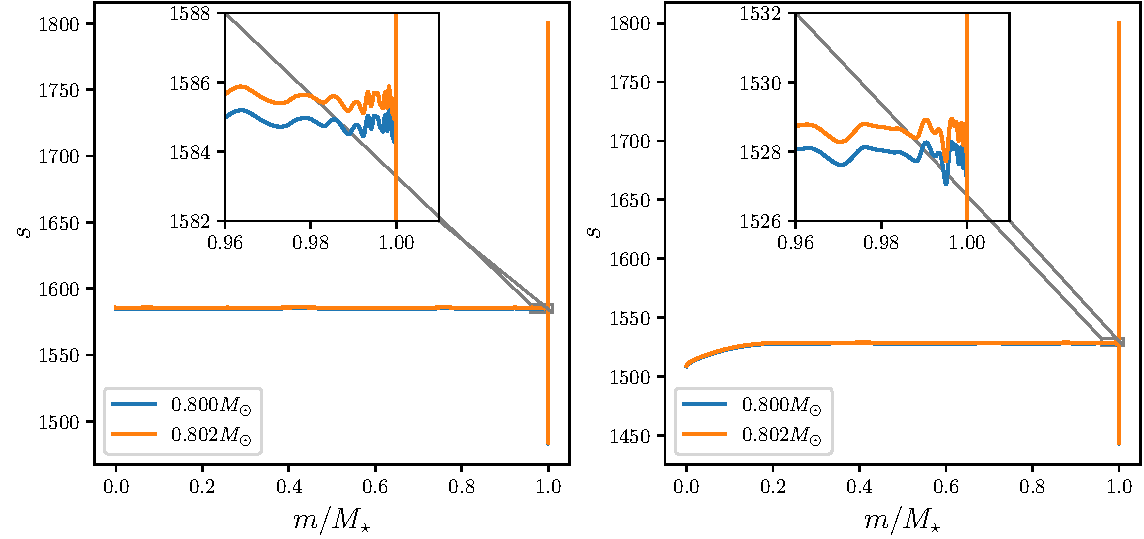
\includegraphics[width=\textwidth,keepaspectratio]{toy_problem_entropy.pdf}
  \caption{Entropy profiles of the static models. The left panel shows the entropy profiles of the two fully convective models, while the right panel shows those of the two models with a radiative core. In both panels, the blue lines correspond to the $0.8\,M_\odot$ models, and the orange lines correspond to the $0.82\,M_\odot$ models.} \label{fig:toy_problem_entropy}
\end{figure}

\subsection{The effect of different initial models}
\label{sec:initial_models}

\subsection{The effect of different accretion rates}
\label{sec:accretion_rate}

\begin{figure}
  \centering  
  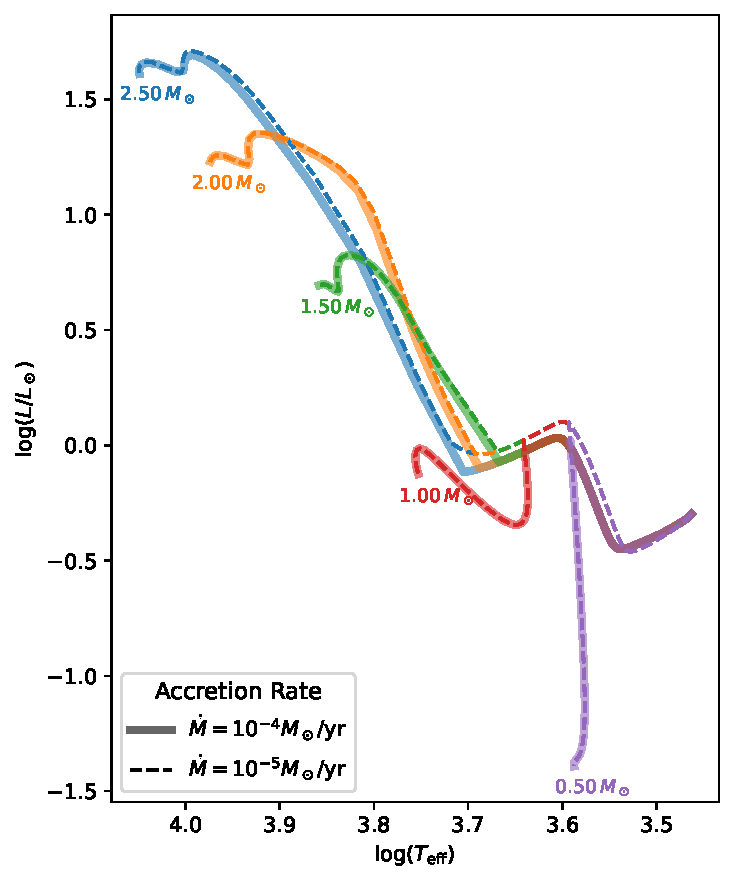
\includegraphics[width=.65\textwidth,keepaspectratio]{comp_accrate.pdf}
  \caption{Comparisons of low-mass accreting models with accretion rates of $10^{-5} M_\odot/\mr{yr}$ (wide, solid lines) and $10^{-4} M_\odot/\mr{yr}$ (thin, dashed lines). The models are initialized with a seed mass of $0.1 M_\odot$ and a deuterium abundance of $\mr{D/H} = 2.0\times 10^{-5}$.} \label{fig:comp_accrate}
\end{figure}

\subsection{The effect of different chemical compositions}
\label{sec:chemical_composition}

\begin{outline}{gray}
  \item compare accreting models with and without deuterium accreted in the outer layers
  \item can try to vary the abundance of deuterium in the accreted material
\end{outline}

\subsection{Comparison with Palla \& Stahler (1993)}
\label{sec:comp_palla_stahler}

\begin{outline}{gray}
  \item try to reproduce a similar plot of Palla \& Stahler (1992) mass-radius relation, or Fig 20.3 in Maeder book
\end{outline}

\begin{figure}
  \centering  
  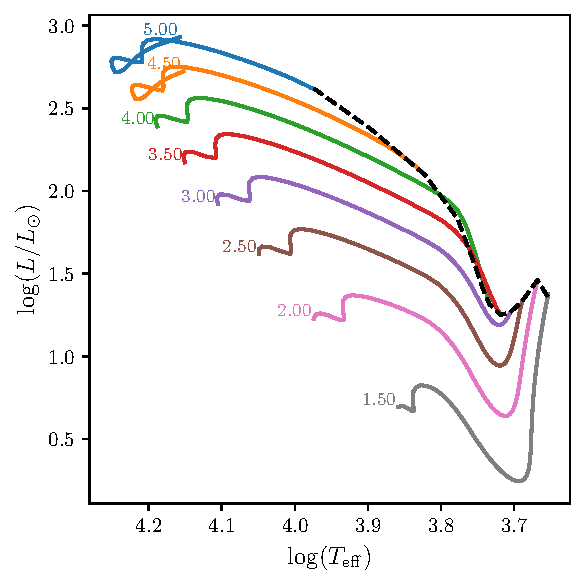
\includegraphics[width=.65\textwidth,keepaspectratio]{birthline_acce5.pdf}
  \caption{Birthline of accreting stars, with an accretion rate of $10^{-5} M_\odot/\mr{yr}$.} \label{fig:birthline_acce5}
\end{figure}

% \subsection{The effect of different initial stellar masses}
% \label{sec:initial_mass}

% \subsection{The effect of different heat injection models}
% \label{sec:heat_injection}

% \subsection{Comparison with \texttt{MESA}}
% \label{sec:mesa_comparison}

\section{Conclusion}
\label{sec:conclusion}

\begin{outline}{gray}
  \item summarize the main findings of the project
  \item discuss the limitations and prospects of this research
  \item limitations of the current implementation
  \begin{itemize}
    \item the seed mass is $0.1 M_\odot$ can be smaller
    \item angular momentum is not considered
    \item variable accretion rate
    \item numeircal treatment of convective-radiative boundary
    \item hot/cold accretion
  \end{itemize}
\end{outline}

% \newpage
% to be done at the end
% \begin{outline}{gray}
%   \item replace pre-main sequence with PMS 
% \end{outline}
% \section*{Acknowledgements}
% \label{sec:acknowledgements}

\newpage
\printbibliography[heading=bibintoc, title={References}]

\newpage
\appendix
\section{Appendix: The jacobian of the stellar structure equations}
\label{sec:appendix_jacobian}
% For simplicity, we will use the following notations:
% \begin{equation*}
%   \xi' \equiv \pfird[\xi]{q},\ \eta' \equiv \pfird[\eta]{q},\ \zeta' \equiv \pfird[\zeta]{q},\ \lambda' \equiv \pfird[\lambda]{q},\ \mu' \equiv \pfird[\mu]{q}
% \end{equation*}

% Derivatives of be(1) with respect to the variables are:
% \begin{align}
%   \text{be(1)}\quad0 &= \pfird[\xi]{q} - \left[-\frac{3G}{8\pi}\left(\frac{M_\odot}{R_\odot}\right)^2\left(\frac{\mu}{\zeta}\right)^2 + \frac{M_\odot}{4\pi R_\odot}\left(\frac{\mu}{\zeta}\right)^{1/2} \Omega^2\right]e^{-\xi}\frac{\psi}{\theta}\\
%   \pfird[\text{(1)}]{\xi} &= -\left[-\frac{3G}{8\pi}\left(\frac{M_\odot}{R_\odot}\right)^2\left(\frac{\mu}{\zeta}\right)^2 + \frac{M_\odot}{4\pi R_\odot}\left(\frac{\mu}{\zeta}\right)^{1/2} \Omega^2\right]\left(-e^{-\xi}\frac{\psi}{\theta}+e^{-\xi}\pfird[(\psi/\theta)]{\xi}\right)\\
%   \pfird[\text{(1)}]{\eta} &= -\left[-\frac{3G}{8\pi}\left(\frac{M_\odot}{R_\odot}\right)^2\left(\frac{\mu}{\zeta}\right)^2 + \frac{M_\odot}{4\pi R_\odot}\left(\frac{\mu}{\zeta}\right)^{1/2} \Omega^2\right]e^{-\xi}\pfird[(\psi/\theta)]{\eta}\\
%   \pfird[\text{(1)}]{\zeta} &= -\left[-\frac{3G}{8\pi}\left(\frac{M_\odot}{R_\odot}\right)^2\left(\frac{\mu}{\zeta}\right)^2 + \frac{M_\odot}{4\pi R_\odot}\left(\frac{\mu}{\zeta}\right)^{1/2} \Omega^2\right]e^{-\xi}\pfird[(\psi/\theta)]{\zeta}\\
%   &\quad -\left[-\frac{3G}{8\pi}\left(\frac{M_\odot}{R_\odot}\right)^2\left(-2\frac{\mu^2}{\zeta^3}\right) + \frac{M_\odot}{4\pi R_\odot}\left(-\frac{1}{2}\frac{\mu^{1/2}}{\zeta^{3/2}}\right) \Omega^2\right]e^{-\xi}\frac{\psi}{\theta}\\
%   \pfird[\text{(1)}]{\lambda} &= -\left[-\frac{3G}{8\pi}\left(\frac{M_\odot}{R_\odot}\right)^2\left(\frac{\mu}{\zeta}\right)^2 + \frac{M_\odot}{4\pi R_\odot}\left(\frac{\mu}{\zeta}\right)^{1/2} \Omega^2\right]e^{-\xi}\pfird[(\psi/\theta)]{\lambda}\\
%   \pfird[\text{(1)}]{\mu} &= -\left[-\frac{3G}{8\pi}\left(\frac{M_\odot}{R_\odot}\right)^2\left(\frac{\mu}{\zeta}\right)^2 + \frac{M_\odot}{4\pi R_\odot}\left(\frac{\mu}{\zeta}\right)^{1/2} \Omega^2\right]e^{-\xi}\pfird[(\psi/\theta)]{\mu}\\
%   &\quad -\left[-\frac{3G}{8\pi}\left(\frac{M_\odot}{R_\odot}\right)^2\left(2\frac{\mu}{\zeta^2}\right) + \frac{M_\odot}{4\pi R_\odot}\left(\frac{1}{2}\frac{\mu^{-1/2}}{\zeta^{1/2}}\right) \Omega^2\right]e^{-\xi}\frac{\psi}{\theta}\\
%   &\pfird[\text{(1)}]{\xi'} = 1,\ \pfird[\text{(1)}]{\eta'} = 0,\ \pfird[\text{(1)}]{\zeta'} = 0,\ \pfird[\text{(1)}]{\lambda'} = 0,\ \pfird[\text{(1)}]{\mu'} = 0,\ \pfird[\text{(1)}]{\psi'} = 0
% \end{align}

% Derivatives of be(2) with respect to the variables are:
% \begin{align}
%   \text{be(2)}\quad0 &= \pfird[\eta]{q} - \left[-\frac{3G}{8\pi}\left(\frac{M_\odot}{R_\odot}\right)^2\left(\frac{\mu}{\zeta}\right)^2 + \frac{M_\odot}{4\pi R_\odot}\left(\frac{\mu}{\zeta}\right)^{1/2} \Omega^2\right]e^{-\xi}\frac{\psi}{\theta}\nabla\\
%   \pfird[\text{(2)}]{\xi} &= -\left[-\frac{3G}{8\pi}\left(\frac{M_\odot}{R_\odot}\right)^2\left(\frac{\mu}{\zeta}\right)^2 + \frac{M_\odot}{4\pi R_\odot}\left(\frac{\mu}{\zeta}\right)^{1/2} \Omega^2\right]\left(e^{-\xi}\nabla\pfird[(\psi/\theta)]{\xi}-e^{-\xi}\nabla\frac{\psi}{\theta} + e^{-\xi}\pfird[\nabla]{\xi}\frac{\psi}{\theta}\right)\\
%   \pfird[\text{(2)}]{\eta} &= -\left[-\frac{3G}{8\pi}\left(\frac{M_\odot}{R_\odot}\right)^2\left(\frac{\mu}{\zeta}\right)^2 + \frac{M_\odot}{4\pi R_\odot}\left(\frac{\mu}{\zeta}\right)^{1/2} \Omega^2\right]e^{-\xi}\left(
%   \nabla\pfird[(\psi/\theta)]{\eta}+\pfird[\nabla]{\eta}\frac{\psi}{\theta}\right)\\
%   \pfird[\text{(2)}]{\zeta} &= -\left[-\frac{3G}{8\pi}\left(\frac{M_\odot}{R_\odot}\right)^2\left(\frac{\mu}{\zeta}\right)^2 + \frac{M_\odot}{4\pi R_\odot}\left(\frac{\mu}{\zeta}\right)^{1/2} \Omega^2\right]e^{-\xi}\left(
%   \nabla\pfird[(\psi/\theta)]{\zeta}+\pfird[\nabla]{\zeta}\frac{\psi}{\theta}\right)\\
%   &\quad -\left[-\frac{3G}{8\pi}\left(\frac{M_\odot}{R_\odot}\right)^2\left(-2\frac{\mu^2}{\zeta^3}\right)+ \frac{M_\odot}{4\pi R_\odot}\left(-\frac{1}{2}\frac{\mu^{1/2}}{\zeta^{3/2}}\right) \Omega^2\right]e^{-\xi}\nabla\frac{\psi}{\theta}\\
%   \pfird[\text{(2)}]{\lambda} &= -\left[-\frac{3G}{8\pi}\left(\frac{M_\odot}{R_\odot}\right)^2\left(\frac{\mu}{\zeta}\right)^2 + \frac{M_\odot}{4\pi R_\odot}\left(\frac{\mu}{\zeta}\right)^{1/2} \Omega^2\right]e^{-\xi}\left(
%   \nabla\pfird[(\psi/\theta)]{\lambda}+\pfird[\nabla]{\lambda}\frac{\psi}{\theta}\right)\\
%   \pfird[\text{(2)}]{\mu} &= -\left[-\frac{3G}{8\pi}\left(\frac{M_\odot}{R_\odot}\right)^2\left(\frac{\mu}{\zeta}\right)^2 + \frac{M_\odot}{4\pi R_\odot}\left(\frac{\mu}{\zeta}\right)^{1/2} \Omega^2\right]e^{-\xi}\left(
%   \nabla\pfird[(\psi/\theta)]{\mu}+\pfird[\nabla]{\mu}\frac{\psi}{\theta}\right)\\
%   &\quad -\left[-\frac{3G}{8\pi}\left(\frac{M_\odot}{R_\odot}\right)^2\left(2\frac{\mu}{\zeta^2}\right)+ \frac{M_\odot}{4\pi R_\odot}\left(\frac{1}{2}\frac{\mu^{-1/2}}{\zeta^{1/2}}\right) \Omega^2\right]e^{-\xi}\nabla\frac{\psi}{\theta}\\
%   \pfird[\text{(2)}]{\psi} &= -\left[-\frac{3G}{8\pi}\left(\frac{M_\odot}{R_\odot}\right)^2\left(\frac{\mu}{\zeta}\right)^2 + \frac{M_\odot}{4\pi R_\odot}\left(\frac{\mu}{\zeta}\right)^{1/2} \Omega^2\right]e^{-\xi}\nabla\frac{1}{\theta}\\
%   &\pfird[\text{(2)}]{\xi'} = 0,\ \pfird[\text{(2)}]{\eta'} = 1,\ \pfird[\text{(2)}]{\zeta'} = 0,\ \pfird[\text{(2)}]{\lambda'} = 0,\ \pfird[\text{(2)}]{\mu'} = 0,\ \pfird[\text{(2)}]{\psi'} = 0
% \end{align}

% Derivatives of be(3) with respect to the variables are:
% \begin{align}
%   \text{be(3)}\quad0 &= \pfird[\zeta]{q} - \frac{3}{4\pi}\frac{M_\odot}{R_\odot^3}\frac{1}{\rho}\left(\frac{\mu}{\zeta}\right)^{1/2}\frac{\psi}{\theta}\\
%   \pfird[\text{(3)}]{\xi} &= - \frac{3}{4\pi}\frac{M_\odot}{R_\odot^3}\left(\frac{\mu}{\zeta}\right)^{1/2}\left(\frac{1}{\rho}\pfird[(\psi/\theta)]{\xi} - \frac{1}{\rho^2}\pfird[\rho]{\xi}\frac{\psi}{\theta}\right)\\
%   \pfird[\text{(3)}]{\eta} &= - \frac{3}{4\pi}\frac{M_\odot}{R_\odot^3}\left(\frac{\mu}{\zeta}\right)^{1/2}\left(\frac{1}{\rho}\pfird[(\psi/\theta)]{\eta} - \frac{1}{\rho^2}\pfird[\rho]{\eta}\frac{\psi}{\theta}\right)\\
%   \pfird[\text{(3)}]{\zeta} &= -\frac{3}{4\pi}\frac{M_\odot}{R_\odot^3}\frac{1}{\rho}\left(\frac{\mu}{\zeta}\right)^{1/2}\pfird[(\psi/\theta)]{\zeta} - \frac{3}{4\pi}\frac{M_\odot}{R_\odot^3}\frac{1}{\rho}\left(-\frac{1}{2}\frac{\mu^{1/2}}{\zeta^{3/2}}\right)\frac{\psi}{\theta}\\
%   \pfird[\text{(3)}]{\lambda} &= -\frac{3}{4\pi}\frac{M_\odot}{R_\odot^3}\frac{1}{\rho}\left(\frac{\mu}{\zeta}\right)^{1/2}\pfird[(\psi/\theta)]{\lambda}\\
%   \pfird[\text{(3)}]{\mu} &= -\frac{3}{4\pi}\frac{M_\odot}{R_\odot^3}\left(\frac{\mu}{\zeta}\right)^{1/2}\left(\frac{1}{\rho}\pfird[(\psi/\theta)]{\mu} - \frac{1}{\rho^2}\pfird[\rho]{\mu}\frac{\psi}{\theta}\right) - \frac{3}{4\pi}\frac{M_\odot}{R_\odot^3}\frac{1}{\rho}\left(\frac{1}{2}\frac{\mu^{-1/2}}{\zeta^{3/2}}\right)\frac{\psi}{\theta}\\
%   \pfird[(3)]{\psi} &= -\frac{3}{4\pi}\frac{M_\odot}{R_\odot^3}\frac{1}{\rho}\left(\frac{\mu}{\zeta}\right)^{1/2}\frac{1}{\theta}\\
%   \pfird[(3)]{\xi'}& = 0,\ \pfird[(3)]{\eta'} = 0,\ \pfird[(3)]{\zeta'} = 1,\ \pfird[(3)]{\lambda'} = 0,\ \pfird[(3)]{\mu'} = 0,\ \pfird[(3)]{\psi'} = 0
% \end{align}

\end{document}
